\documentclass[12pt]{article}

\usepackage{fixltx2e}
\usepackage{textcomp}
\usepackage{fullpage}
\usepackage{amsfonts}
\usepackage{verbatim}
\usepackage[english]{babel}
\usepackage{pifont}
\usepackage{color}
\usepackage{setspace}
\usepackage{lscape}
\usepackage{indentfirst}
\usepackage[normalem]{ulem}
\usepackage{booktabs}
% \usepackage{nag}
\usepackage{natbib}
% \usepackage{bibtex}
\usepackage{float}
\usepackage{latexsym}
\usepackage{hyperref}
\usepackage{url}
% \usepackage{html}
\usepackage{epsfig}
\usepackage{graphicx}
\usepackage{amssymb}
\usepackage{amsmath}
\usepackage{bm}
\usepackage{array}
%\usepackage{mhchem}
\usepackage{ifthen}
\usepackage{caption}
\usepackage{xcolor}
\usepackage{amsthm}
\usepackage{amstext}
\usepackage{nicefrac}
\usepackage{algorithm}
\usepackage{algorithmic}
\usepackage[scientific-notation=true]{siunitx}
\usepackage{subfigure}
\usepackage[flushleft]{threeparttable}
\usepackage{lineno}
\usepackage{adjustbox}
\usepackage{ragged2e}

\setlength{\parskip}{1em}
\renewcommand{\baselinestretch}{2.0}

\begin{document}

\begin{minipage}[h]{\textwidth}
	\title{StarBEAST2 enables accurate and precise inference of species trees, divergence times and clock rates}
	\author{Huw A. Ogilvie$^{\ast,1,2}$ and Alexei J. Drummond,$^{2,3}$}
    \maketitle
\end{minipage}

\raggedright
$^{1}$Department of Evolution, Ecology and Genetics, Australian National University, Canberra, Australia\\
$^{2}$Centre for Computational Evolution, University of Auckland, Auckland, New Zealand\\
$^{3}$Department of Computer Science, University of Auckland, Auckland, New Zealand

\clearpage

\justifying

\section{Abstract}

Keywords: Phylogenetic methods, substitution rate, relaxed clock, multispecies coalescent, concatenation.

\section{Introduction}


\section{New Approaches}

\subsection{Coordinated tree changing operators}

\subsection{Species tree relaxed clocks}

\section{Results}

\subsection{StarBEAST2 correctly implements the multispecies coalescent}

New methods must be shown to be mathematically correct implementations of a
given model. One way to accomplish this for MCMC methods is to estimate
parameters from a prior distribution using the MCMC kernel, and also draw
independent samples from the same prior distribution by simulation. The
resulting parameter distributions should be identical if the implementation is
correct. We used this method to test the correctness of the novel features in
StarBEAST2; analytical population size integration, the four new operators, and
the species tree relaxed clock. Simulated and StarBEAST2 estimated distributions
were identical for species and gene tree topologies (Figure~S1,S2), species and
gene tree node heights (Figure~S3,S4) and gene tree branch rates (Figure~S5).
This combination of results supports the mathematical correctness of StarBEAST2.

\subsection{North American chorus frogs have intermediate coalescent branch lengths}

To determine which configuration of new features would achieve the fastest
performance, we ran StarBEAST2 using different combinations of new operators,
analytical integration of population sizes and relaxed clocks. The sequence data
used for this analysis is from the North American chorus frog genus
\textit{Pseudacris} originally collected and analyzed by \cite{Barrow201478}. A
key metric of phylogenies that determines the necessity of multispecies
coalescent models is the average branch length in coalescent units of
$\nicefrac{\tau}{2Ne}$. Given short branch lengths, concatenation is unable to
infer accurate species trees regardless of the number of loci used. Given long
branch lengths, concatenation is approximately as accurate as the multispecies
coalescent \citep{Ogilvie01052016}. Using StarBEAST2, the average branch length
within this genus was determined to be $\nicefrac{1.69\tau}{2Ne}$. This is an
intermediate average length compared to the shallow simulations analyzed by
\cite{Ogilvie01052016}, which had short branch lengths of
$\nicefrac{0.54\tau}{2Ne}$.

\subsection{New operators and analytical integration improve computational performance}

To measure convergence both effective sample size (ESS) per hour and ESS per
million states were computed for each independent chain. ESS per hour can be
used calculate the total time required for a converged chain where ESS is equal
to or above 200, and reflects the efficiency of new state proposals and the
computational time required by each operator and likelihood calculation. In
contrast, ESS per million states reflects only to the efficency of new state
proposals, independent of calculation times. A variety of statistics were logged
for each analysis, but the height of the species tree had the slowest
convergence rates so we used this statistic to judge computational performance
(Figure~S7-Sx).

Coordinated topology operators consistently reduced ESS per hour convergence,
regardless of the addition of height changing operators or the method of
population size integration (Figure~\ref{fig:realEssPerHour}). However these
operators had little effect on ESS per million states (Figure~\ref{fig:realEssPerMstates}).
The latter result suggests that coordinated topology operators are not more
effective than na\"ive operators at proposing new states, and the former result
shows how the increased complexity of these operators harms convergence because
of their increased computational time cost.

Coordinated height changing operators consistently improved convergence both in terms
of ESS per hour and ESS per million states (Figure~\ref{fig:realEssPerHour},\ref{fig:realEssPerMstates}).
Both species tree relaxed clock and gene tree relaxed clock analyses benefitted
from enabling these new operators. Analytical integration of population sizes
improved the computational performance of gene tree relaxed clock analyses, but
not species tree relaxed clock analyses.

Convergence of species tree relaxed clock analyses was dramatically slower than
convergence of gene tree relaxed clock analyses, both in terms of ESS per hour
and ESS per million states
(Figure~\ref{fig:realEssPerHour},\ref{fig:realEssPerMstates}).

\begin{figure}[htb!]
\centering
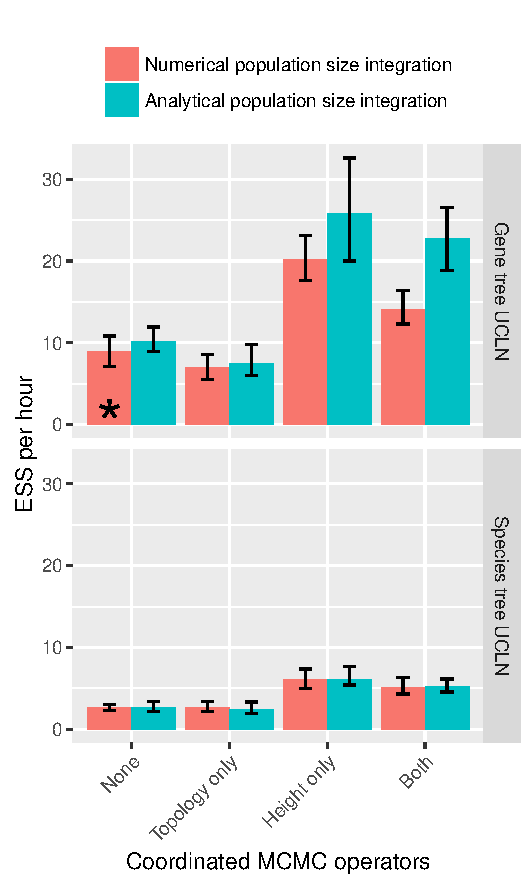
\includegraphics[height=14cm]{speciesTreeHeight_ess_per_hour.pdf}
\caption
{Effect of operators, population size integration and clock models on
convergence. The performance of every combination of settings was measured when
applied to 22 \textit{Pseudacris} loci. Topology operators refers to the
replacement of na\"ive NNI and SPR operators with coordinated operators. Heights
operators refers to the addition of operators which make coordinated changes to
internal node heights. Uncorrelated lognormal (UCLN) relaxed clocks were applied
to either each gene tree or to the species tree. Trimmed means of species tree
height effective sample size (ESS) per hour were calculated from 32 independent
chains. 25\% trim was used to reduce the influence of outliers. All error bars
are 95\% confidence intervals calculated by bootstrapping.}
\label{fig:realEssPerHour}
\end{figure}

\begin{figure}[htb!]
\centering
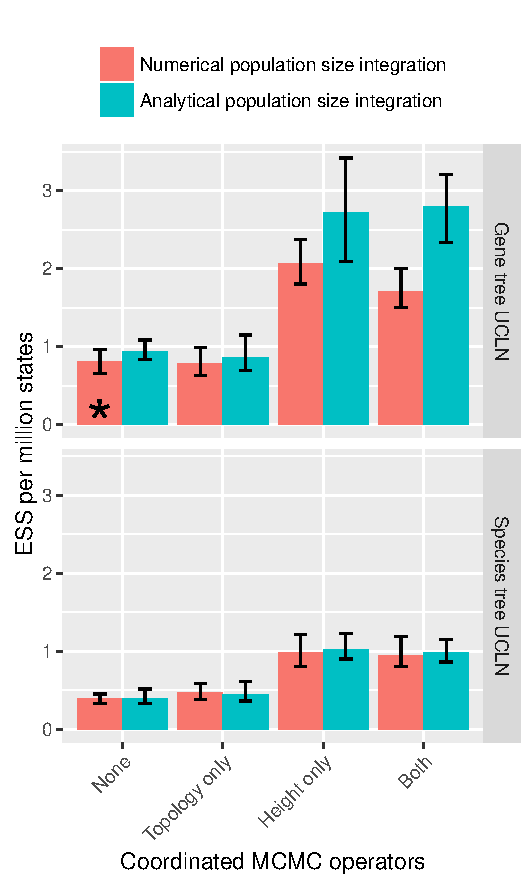
\includegraphics[height=14cm]{speciesTreeHeight_ess_per_mstates.pdf}
\caption
{Effect of operators, population size integration and clock models on effective
sample size (ESS) per million states. The performance of every combination of
settings was measured when applied to 22 \textit{Pseudacris} loci. Topology operators refers to the
replacement of na\"ive NNI and SPR operators with coordinated operators. Heights
operators refers to the addition of operators which make coordinated changes to
internal node heights. Uncorrelated lognormal (UCLN) relaxed clocks were applied
to either each gene tree or to the species tree. Trimmed means
of species tree height ESS per million states were calculated from 32
independent chains. 25\% trim was used to reduce the influence
of outliers. All error bars are 95\% confidence intervals calculated by
bootstrapping.}
\label{fig:realEssPerMstates}
\end{figure}

\clearpage

\begin{figure}[htb!]
\centering
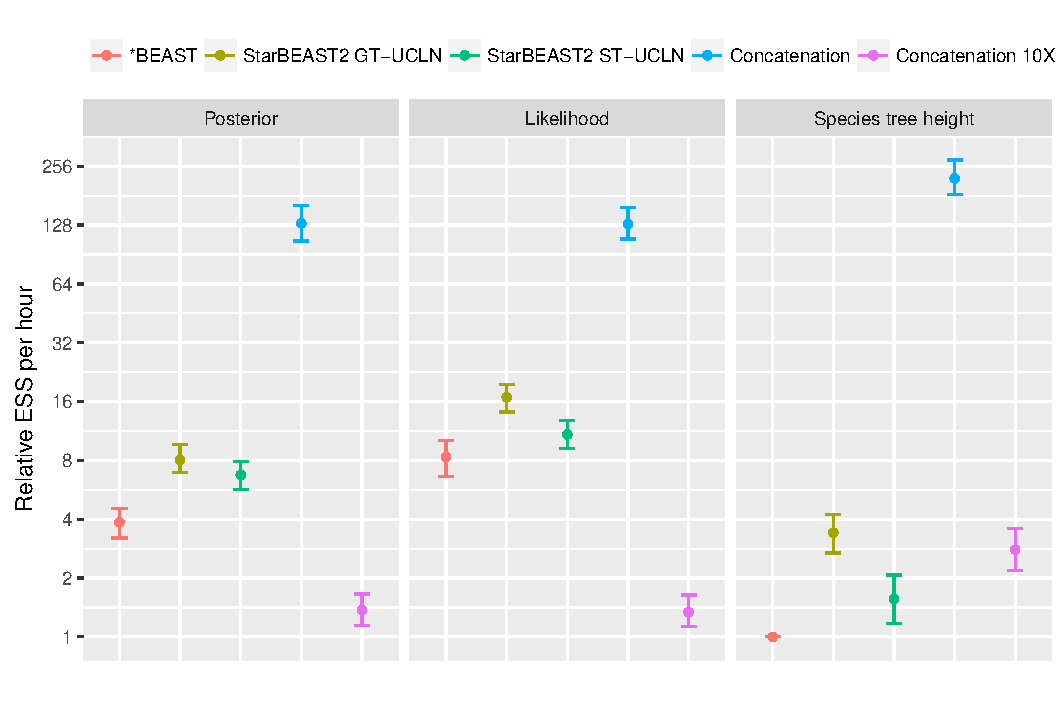
\includegraphics[width=16cm]{multiple_ess_per_hour.pdf}
\caption
{Convergence of different methods applied to simulated data. Methods are
concatenation with 22 loci, concatenation with 220 loci (10X), StarBEAST2 with
*BEAST settings and 22 loci, and StarBEAST2 with performant settings, 22 loci,
and uncorrelated lognormal relaxed clocks applied to the gene tree (GT-UCLN) or
to the species tree (ST-UCLN). Relative ESS per hour is the trimmed mean of
effective sample size per hour for each replicate divided by the slowest rate
--- that of the species tree height estimated by StarBEAST2 with *BEAST
settings. 25\% trim was used to reduce the influence of
outliers. All error bars are 95\% confidence intervals calculated by
bootstrapping. N = 64.}
\label{fig:simulatedEssPerHour}
\end{figure}

\clearpage

\begin{figure}[htb!]
\centering
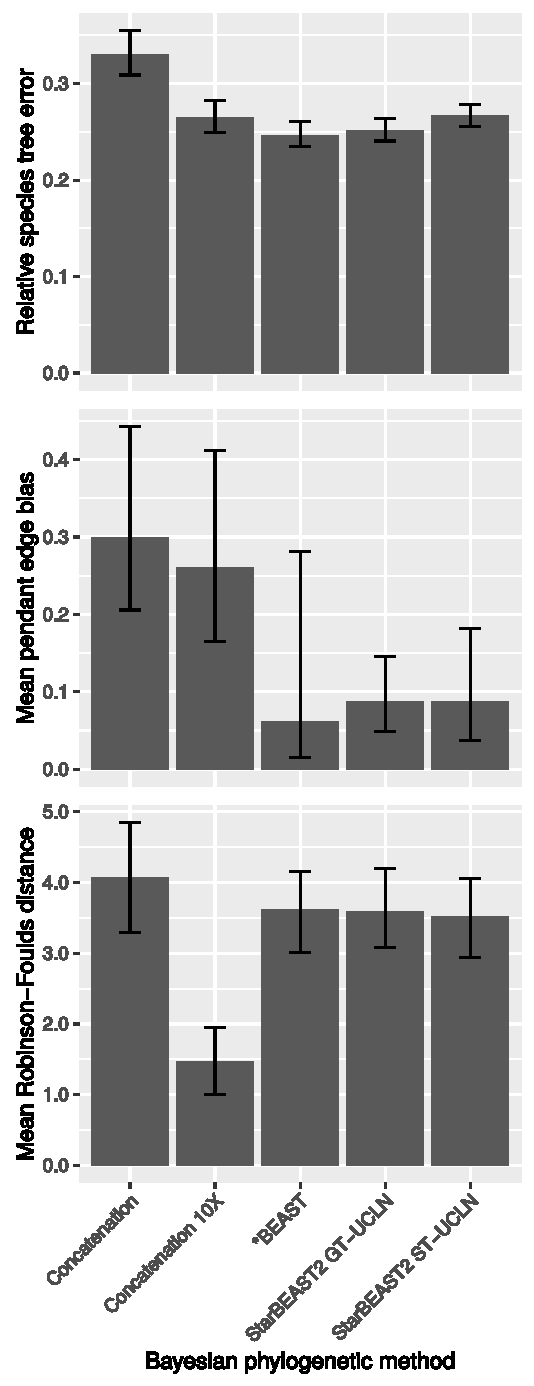
\includegraphics[width=6.5cm]{tree_error.pdf}
\caption
{Accuracy of different methods applied to simulated data. Methods are concatenation with 22 loci, concatenation with 220 loci
(10X), StarBEAST2 with *BEAST settings and 22 loci, and StarBEAST2 with
performant settings, 22 loci, and uncorrelated lognormal relaxed clocks applied
to the gene tree (GT-UCLN) or to the species tree (ST-UCLN). (A) Trimmed mean of
relative species tree error, a measure of branch length error. (B) Trimmed
mean of mean pendant edge bias, which measures biased estimates of the ages of
extant species. (C) Trimmed mean of mean rooted Robinson-Foulds distances, a
measure of topological error. 25\% trim was used to reduce the
influence of outliers. All error bars are 95\% confidence intervals calculated
by bootstrapping. N = 64.}
\label{fig:speciesTreeError}
\end{figure}

\clearpage

\begin{figure}[htb!]
\centering
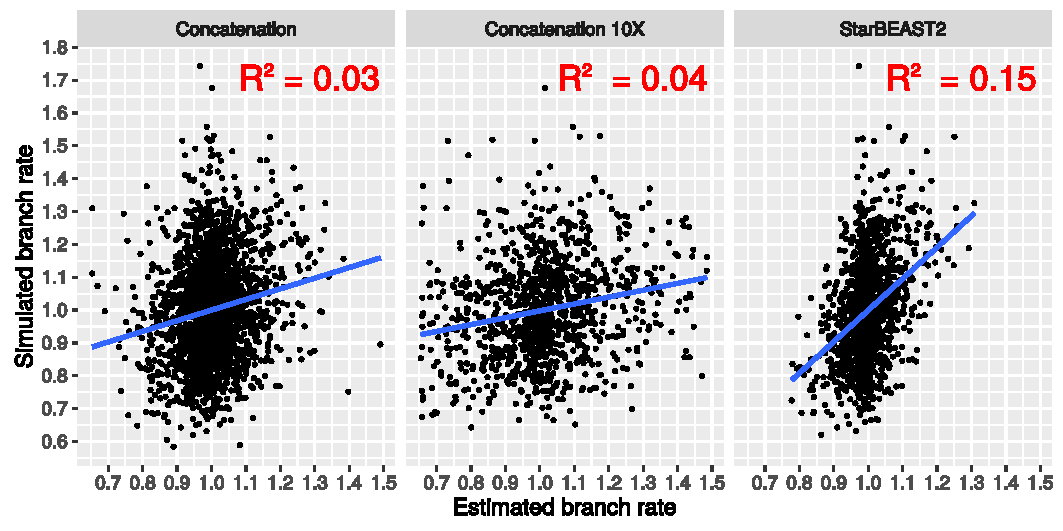
\includegraphics[width=16cm]{branch_rates_lm.pdf}
\caption
{Recovery of species tree branch rates using concatenation and StarBEAST2.
Methods are concatenation with 22 loci, concatenation with 220 loci (10X), and
StarBEAST2 with performant settings, 22 loci, and an uncorrelated lognormal
relaxed clocks applied to the species tree (ST-UCLN). Estimated rates are the
posterior expectation of the branch rate conditional on the monophyly of the
corresponding clade. $R^2$ values and lines of best fit were calculating using a separate
simple linear regression for each method. Root branch rates, which were fixed at
1.0, were excluded. N = 64.}
\label{fig:branchRatesLM}
\end{figure}

\clearpage

\section{Discussion}


\section{Materials and Methods}


\section{Supplementary Material}
Supplementary tables XX-XX and figures XX-XX are available at \textit{Molecular Biology and Evolution} online (http://www.mbe.oxfordjournals.org/).


\section{Acknowledgments}
Blah blah blah


\bibliographystyle{natbib}
\bibliography{starbeast2}

\end{document}
